\documentclass[final,t]{beamer}
\mode<presentation>
{
%  \usetheme{Warsaw}
%  \usetheme{Aachen}
%  \usetheme{Oldi6}
%  \usetheme{I6td}
  \usetheme{I6dv}
%  \usetheme{I6pd}
%  \usetheme{I6pd2}
}
% additional settings
\setbeamerfont{itemize}{size=\normalsize}
\setbeamerfont{itemize/enumerate body}{size=\normalsize}
\setbeamerfont{itemize/enumerate subbody}{size=\normalsize}

% additional packages
\usepackage{times}
\usepackage{amsmath,amsthm, amssymb, latexsym}
\usepackage{exscale}
\usepackage{multirow}
%\boldmath
\usepackage{booktabs, array}
%\usepackage{rotating} %sideways environment
\usepackage[english]{babel}
\usepackage[latin1]{inputenc}
\usepackage[orientation=landscape,size=custom,width=300,height=200,scale=2.6]{beamerposter}
\listfiles
\graphicspath{{figures/}}
% Display a grid to help align images
%\beamertemplategridbackground[1cm]

\title{\huge Automatic Spike Sorting: Visualizing Massive Data Sets}
\author{David Brody}
\institute[Stanford University]{Department of Computer Science,
  Stanford University, Stanford, California}
\date[Dec. 10 , 2011]{Dec. 10 , 2011}

% abbreviations
\usepackage{xspace}
\makeatletter
\DeclareRobustCommand\onedot{\futurelet\@let@token\@onedot}
\def\@onedot{\ifx\@let@token.\else.\null\fi\xspace}
\def\eg{{e.g}\onedot} \def\Eg{{E.g}\onedot}
\def\ie{{i.e}\onedot} \def\Ie{{I.e}\onedot}
\def\cf{{c.f}\onedot} \def\Cf{{C.f}\onedot}
\def\etc{{etc}\onedot}
\def\vs{{vs}\onedot}
\def\wrt{w.r.t\onedot}
\def\dof{d.o.f\onedot}
\def\etal{{et al}\onedot}
\makeatother

%%%%%%%%%%%%%%%%%%%%%%%%%%%%%%%%%%%%%%%%%%%%%%%%%%%%%%%%%%%%%%%%%%%%%%%%%%%%%%%%%%%%%%%%%%%%%%%%%%%%%%%%%%%%
%%%%%%%%%%%%%%%%%%%%%%%%%%%%%%%%%%%%%%%%%%%%%%%%%%%%%%%%%%%%%%%%%%%%%%%%%%%%%%%%%%%%%%%%%%%%%%%%%%%%%%%%%%%%
\begin{document}
\begin{frame}{} 
  \begin{columns}[t]
    \begin{column}{.3\linewidth}

      %%%%%%%%%%%%%%%%%%%%%%%%%%%%%%%%%%%%%%%%%%%%%%%%%%%%%%%%%%%%%%%%%%%%%%%%%%%%%%%%%%%%%%%%%%%%%%%%%%%%%%%%%%%%

      \begin{block}{Introduction}
             This project is aimed to create software to 
             \alert{help neuroscientists analize their
               electrophysiological data}. Specifically, this software was designed to help automate
             the currently tedious task of spike sorting within the
             Baccus Lab. The software takes the output of an automatic
             spike sorter and allows the scientist to explore and modify
             the data as well as save and load their
             sessions. Finally, it allows the user to export their
             work for further analysis using other tools.
       \end{block}

      %%%%%%%%%%%%%%%%%%%%%%%%%%%%%%%%%%%%%%%%%%%%%%%%%%%%%%%%%%%%%%%%%%%%%%%%%%%%%%%%%%%%%%%%%%%%%%%%%%%%%%%%%%%%

       \begin{block}{Problem and Data Description }
        
         Learning how the data is collected and what it represents
         is crutial to ensure the software address the challenge
         correctly. The data is collected during a wet experiment in which the
         scientist disects a salamander and places a retina on a
         microelectrode array. The many ganglion
         cells of the retina are then stimulated with visual
         stimulus causing them to spike. All the spikes from a
         single cell have a similar shape however each cell may
         have a different shape. Three example spike shapes may
         look like:
         \vskip1em
         \begin{table}[ht]
           \centering
           \begin{tabular}{c c c }
             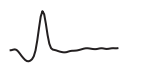
\includegraphics[width=0.2\linewidth]{images/WaveShape1.png} &
             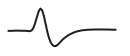
\includegraphics[width=0.2\linewidth]{images/WaveShape2.png} &
             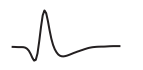
\includegraphics[width=0.2\linewidth]{images/WaveShape3.png}
           \end{tabular}
         \end{table}
         \begin{center}
         \end{center}
         \vskip1em
         Each electrode on the array constantly records the voltage
         at its point at a rate of 10KHz. However, since the
         recording is extracellular it picks up the voltage traces
         of many neighboring cells. A sample recording from an
         electrode may look like the following:
         \vskip1em
         \begin{center}
           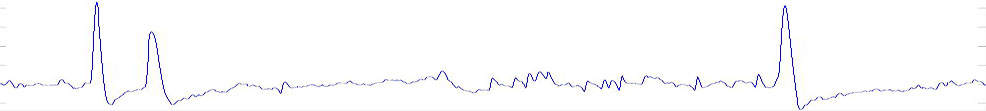
\includegraphics[width=0.8\linewidth]{images/voltagetrace_2_small.jpg}
         \end{center}
         \vskip1em
         This data is then fed into an automatic sorter which
         pulls the spikes out of the data stream and into clusters
         which may be cells. Taking each cluster and overlaying each
         spikeshape gives the following examples of what the dataset includes:
         \vskip1em
         \begin{table}[ht]
           \centering
           \begin{tabular}{c c  c }
             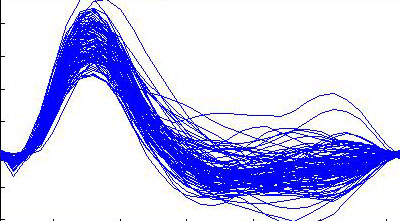
\includegraphics[width=0.2\linewidth]{images/spikeshape_1_small.jpg}
             &
             \hskip3cm  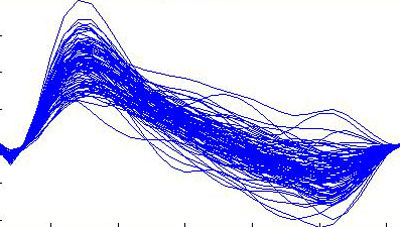
\includegraphics[width=0.2\linewidth]{images/spikeshape_2_small.jpg} &
             \hskip3cm 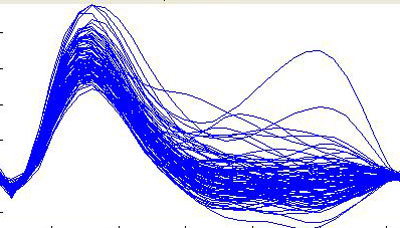
\includegraphics[width=0.2\linewidth]{images/spikeshape_3_small.jpg}
           \end{tabular}
         \end{table}
         \vskip1em
         The scientists want to make sure that certain
         properties of each cluster are correct before they accept it
         as a potential cell to further analize. The tool presented
         here aims to help them explore and refind the data.
       \end{block}
       
       \begin{block}{Other Current Solutions}
         \vskip1em
         \begin{table}
           \begin{tabular}{p{25cm} p{5cm} l}
             \multirow{7}{*}{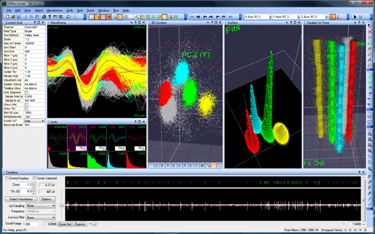
\includegraphics[width=1.0\linewidth]{images/plexon_01.jpg}}
             & & - Limited To 3 Electrodes (max) \\ 
             & & + Great 3d Visualizations \\
             & & + Real Time Interactive \\ 
             & &  - Not Matlab \\
             & & \\
             & & \\
             & & \\
          \end{tabular}
         \end{table}
        
         \begin{table}
           \begin{tabular}{p{25cm} p{5cm} l}
             \multirow{6}{*}{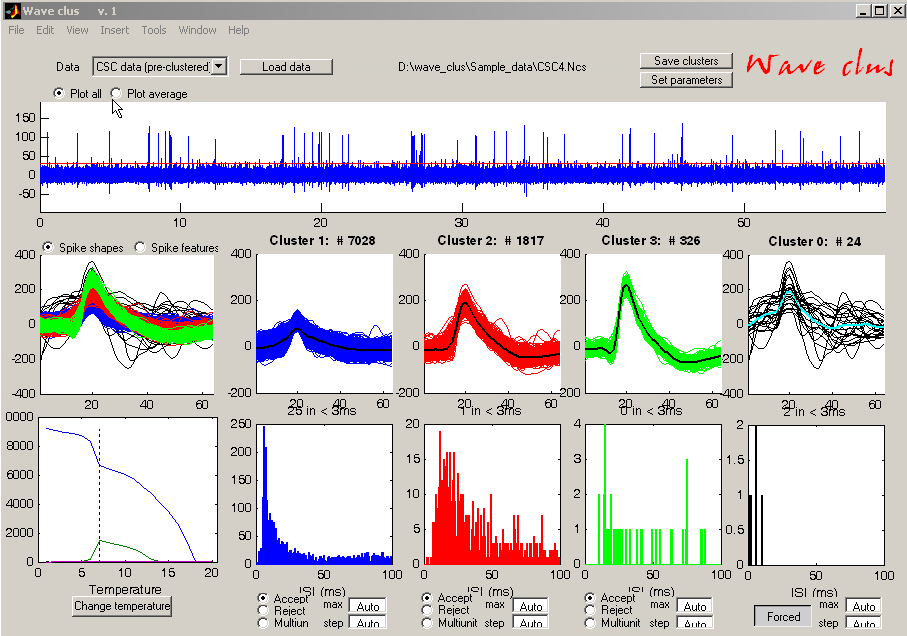
\includegraphics[width=1.0\linewidth]{images/wave_clus.png}}
             &  & - Limited To 5 clusters (max) \\ 
             & & - Not Real Time Interactive \\
             & &  + Matlab \\
             & & \\
             & & \\
             & & \\
          \end{tabular}
         \end{table}
        
         \vskip3cm
         
     \end{block}

      %%%%%%%%%%%%%%%%%%%%%%%%%%%%%%%%%%%%%%%%%%%%%%%%%%%%%%%%%%%%%%%%%%%%%%%%%%%%%%%%%%%%%%%%%%%%%%%%%%%%%%%%%%%%
      

      %%%%%%%%%%%%%%%%%%%%%%%%%%%%%%%%%%%%%%%%%%%%%%%%%%%%%%%%%%%%%%%%%%%%%%%%%%%%%%%%%%%%%%%%%%%%%%%%%%%%%%%%%%%%

    \end{column}
    \begin{column}{.3\linewidth}
      



      \begin{block}{Univariate Class Label Potentials}
        \vfill
        \noindent{\textbf{Features}}
        \begin{itemize}
        \item Person \alert{node degree} - ${0, 1, 2, ...}$
        \item Average outgoing \alert{email length} - discretized into 31 intervals
        \item Ratio of outgoing emails - $\frac{\#sent}{\#sent +
            \#recieved}$ discretized in 4 bins by 0.25
        \item 1936 \alert{subject title} word indicators - binary random variables
        \end{itemize}
        \vskip1ex
        \noindent{\textbf{Clustering}}
        \begin{itemize}
          \item Trained using various amounts of clusters {7,...,15}
          \item Compared Log Likelihood and BIC
        \end{itemize}

        \vskip1ex
        \noindent{\textbf{Feature Strengths}}
         \begin{table}
          \centering
          %\footnotesize
          %\caption{Baseline results using appearance-based features}
          \begin{tabular}{@{} p{.6\linewidth} r r r @{}}
            \toprule
            Word & Rank & Count  & \space Score$^1$ \\
            \midrule
            testimony & 1 & 12 & 1.0499 \\
            sac & 2 & 5 & 0.9934 \\
            website & 8 & 19 & 0.8036 \\
            ... \\
            status & 1933 &  79 & 0.00017 \\
            investments & 1934 & 5 & 0.00017 \\
            2 & 1935 & 132 & 0.00015 \\
            crude & 1936 & 8 & 0.00015 \\
          \bottomrule
          \end{tabular}
          \label{tab:baseline-results}
        \end{table}
        \small{$^1$ Score is variance of resulting CPD}
      \end{block}

      

      \begin{block}{Univariate Link Activity Potentials}
         \noindent{\textbf{Overview}}\par
          Allows us to \alert{incorporate structure} of social graph of
             the training data by assigning a $\gamma_{ij}(Y_{ij})$
         \vskip1ex
         \noindent{\textbf{Method}}\par
         Define $\gamma_{ij}(Y_{ij})$ for $1 \le i \le j \le n$ by:
         \begin{itemize}
         \item $\gamma_{ij}(0) = 1$
         \item $\gamma_{ij}(1) = 1 + score(i,j)$
         \end{itemize}
         \vskip1ex
         Various $score(i,j)$ definitions:
         \begin{itemize}
           \item Common Neighbors Score
           \item Jaccard coefficient score
           \item Zero Score (Uniform)
           \end{itemize}
      \end{block}

      \begin{block}{Triangle Template Potentials}
         \noindent{\textbf{Overview}}\par
         \begin{itemize}
           \item Use training data as \alert{instantiation of unrolled
          network} to observe $Y_{ij}$ then complete data using $C_i = c_i^* = \arg\max_{c_i} \phi_i(c_i)$ for every $i$.
          \item Gradient ascent for parameters of $\psii(c_i,c_j,y)$
            intractable since it requires inference over the joint assignment to all
         variables in $\mathcal X$. 
        \end{itemize}inference
         \vskip1ex
         \noindent{\textbf{Method 1}}\par
         \begin{itemize}
           \item Used \alert{hard assignment} to $\phi_i(C_i)$ since
             potentials usually assign high probability to a single class.
           \item Gradient of (conditional) likelihood becomes more tractable:
          \[ \frac {\partial} {\partial w_{c_1, c_2, y}} \frac 1 M \ell(\bm \theta : \mathcal D) = \frac 1 M M[c_1, c_2, y] - P(c_1, c_2, y) \]
           \item No inference or gradient ascent by setting to 0.
         \end{itemize}
         \vskip1ex
         \noindent{\textbf{Method 2}}\par
         \begin{itemize}
           \item Network distribution is represented as 
             \[ P(\mathcal X) = \frac 1 {Z} \left( \prod_i \phi_i(C_i) \right) \left( \prod_{i < j} \psi(C_i, C_j, Y_{ij}) \right) \left( \prod_{i < j} \gamma_{ij}(Y_{ij})) \right)\]
           \item Structure creates correspondence between
             $\phi(C_i,C_j,Y_{ij})$ and $P(Y_{ij} | C_i, C_j)$
           \item Learn $\bm \theta$ as entires of CPD for $P(Y |
             C_i,C_j)$ 
          \end{itemize}
       \end{block}

    \end{column}

    %%%%%%%%%%%%%%%%%%%%%%%%%%%%%%%
    
    \begin{column}{.3\linewidth}
      
       \begin{block}{Model Querying}
        \begin{itemize}
        \item Run \alert{loopy belief propigation} to obtain marginal
          distributions for $P(C_i)$ and $P(Y_{ij})$ for all $i$ and
          $j$.
          \item Structure is similar to Bethe construction
          \item Graph is family preserving and satifies running
            intersection property.
        \end{itemize}
      \end{block}


     \begin{block}{Experimental Results}
We focussed our comparison on two specific predictors, common
neighbors and Jaccard’s coefficient.
\break
\begin{center}
\begin{tabular}{p{.8\linewidth} |c}
\hline
\textsc{Prediction Method} & \textsc{Accuracy} \\
\hline
\hline
Common neighbors & 0.1407
\\
Jaccard coefficient & 0.1759
\\
Random guessing & 0.0194
\\
\\
Full inference method 1; Common Neighbor link potentials & 0.1407
\\
Full Inference method 1; Jaccard link potentials & 0.1759                     %0.17588
\\
Full Inference method 1; Trivial link potentials & 0.0151                     %0.0151
\\
\\ % trial 2 = V structure
Full inference method 2; Common Neighbor link potentials & 0.1206
\\
Full inference method 2; Jaccard Score link potentials & 0.0402               %0.040201
\\
Full inference method 2; Trivial link potentials & 0.0201                     %0.020101
\\
\\ % conditional inference = with evidence.  V structure is used
Full conditional inference; Common Neighbor link potentials & 0.1206
\\
Full conditional inference; Jaccard link potentials & \textbf{0.1859}
\\
Full conditional inference; Trivial link potentials & 0.0251                 %0.0025126
\\
\hline
\end{tabular}
\end{center}
\vskip1ex

High score of  method 1 with nontrivial link potentials accuracy led to believe \alert{triangle template
factors were contributing little useful information}.
\break
\break
Tested link prediction with triangle template potentials alone with
and without link potentials:
\break
\begin{center}
\begin{tabular}{l|c}
\hline
\textsc{Prediction Method} & \textsc{Accuracy} \\
\hline
\hline
Triangle template potential trial 1; Trivial link potential & 0.0201
\\
Triangle template potential trial 1; Common Neighbor link potential & 0.0754                    %0.075377
\\
Triangle template potential trial 1; Trivial link potential, 3 classes & 0.0302                                                  %0.030151
\\
Triangle template potential trial 1; Common Neighbor link potential, 3 classes & 0.0905     %0.090452
\\
Triangle template potential trial 2; Trivial link potential & 0.0201
\\
Triangle template potential trial 2; Common Neighbor link potential & 0.0754
\\
\hline
\end{tabular}
\end{center}

\break
      \end{block}
                
      \begin{block}{Conclusion}
        \vskip1ex
        \noindent{\textbf{Conclusions}}
        \begin{itemize}
        \item Achieved result close to graph-structure based link predictors
        \item Experiments show that success of prediction comes from
          having \alert{accurate univariate link potential}
         \item Model preserves information
          \item \alert{Adding classifications of people does not significantly
          add to predictive power}
          \begin{itemize}
            \item May be because Email is poor indicator of useful
              class partitioning
            \end{itemize}
        \end{itemize}

        \vskip1ex
        \noindent{\textbf{Learnings}}
        \begin{itemize}
        \item Make sure features chosen have \alert{suffient
          mutual informtion} with variables of interest 
        \end{itemize}

        \vskip1ex
        \noindent{\textbf{Future Work}}
        \begin{itemize}
          \item Try with features of email that may be more indicitive
            of future communications
          \item Try in domain that has \alert{more direct features} of who a
            person may communicate with
            \begin{itemize}
              \item Facebook information would allow for application
                to social network structure as well as indicitive
                features of each person including location, school,
                interests, etc.
            \end{itemize}
          \item Test model in scenario where limited amounts of test
            data are observable
         \end{itemize}

        \vspace{-1ex}
      \end{block}
%%%%%%%%%%%%%%%%%%%%%%%%%%%%%%%%%%%%%%%%%%%%%%%%%%%%%%%

    \end{column}
  \end{columns}
\end{frame}

\end{document}


%%%%%%%%%%%%%%%%%%%%%%%%%%%%%%%%%%%%%%%%%%%%%%%%%%%%%%%%%%%%%%%%%%%%%%%%%%%%%%%%%%%%%%%%%%%%%%%%%%%%
%%% Local Variables: 
%%% mode: latex
%%% TeX-PDF-mode: t
%%% End: 
